Preliminary workshops were conducted to explore the design space of \todo{ad hoc interfaces} in the home environment.
The intend was to get a deeper understanding of how regular users, the participants, interact with products in their home and to explore the potential in the notion of \todo{ad hoc interfaces}.

\section{Workshop approach}

Our approach to the workshops was inspired by different elements from the literature. \todo{\dots}

We chose to conduct the workshops in the homes of the participants as it of course is a very familiar setting where the participants would \hl{be on top and not feel as guests ...}

\subsection{Fictional space}

\todo{what is fictional space}

When trying to explore though interactions and situations it can be beneficial to scope the setting by staging a concrete and limited scenario which participants can adhere to.

\todo{creating obstructions and staging the situation.}

\subsection{Inspiration cards}

illustrative cards on metaphores and technology.

\subsection{Props}

\todo{mangler bl.a. at bringe teori p\aa \ banen}

In preparation for the workshops we collected a variety of different props that could potentially be useful mediators during the workshops.
The intention here was to have artefacts that could spur imagination amongst the participants and help stage the fictional spaces created.

Figure ~\ref{ch:workshops:props-box} shows a box with the props chosen for the workshops.

\begin{itemize}
  \item{Pen, paper(A3, A4), Post-Its, white board foil and transparencies for sketching, drawing and note-taking.}
  \item{Different fabrics like cloth and a fabric-surface mousepad for their flexible characteristics.}
  \item{Plasticine for direct manipulation and for moulding different shapes}
  \item{Rigid objects which could have imaginative behaviour and functionality.}
\end{itemize}

\begin{figure}[hb]
  \centering
    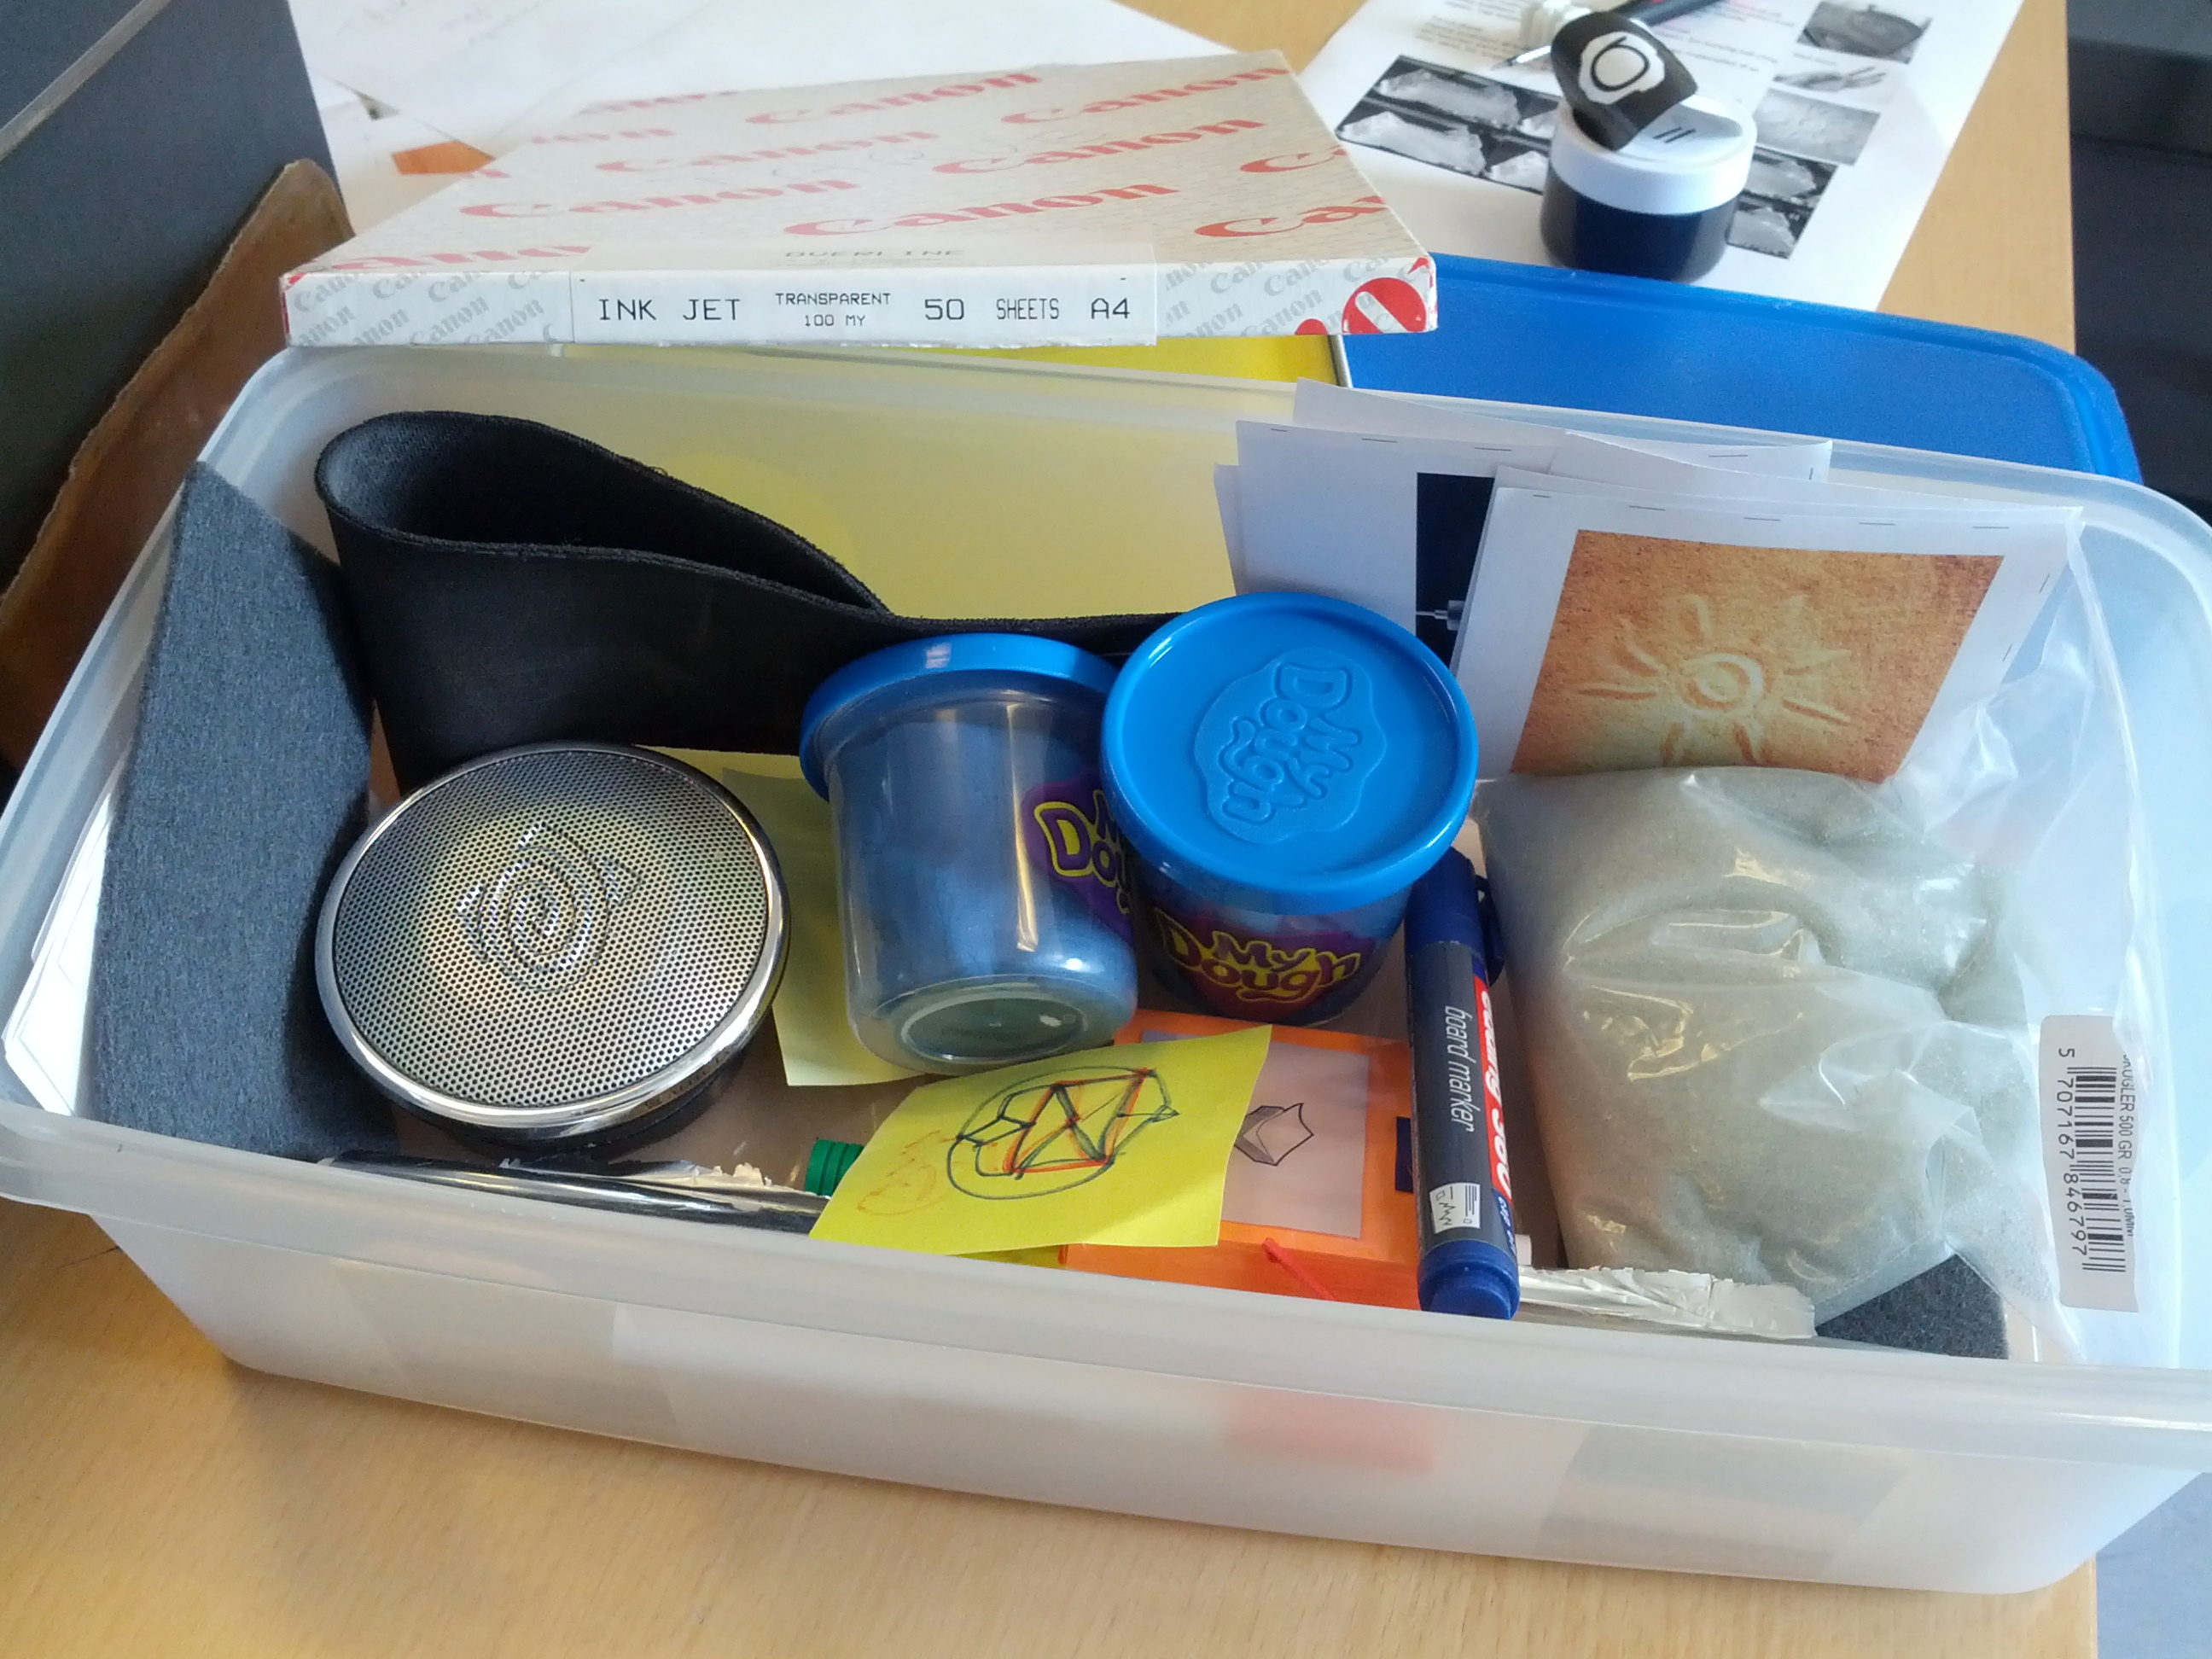
\includegraphics[width=4in]{workshops/props-box}
    \caption[A box with a variety of workshop props.] % in list of figures
  {The box with a variety of workshop props.} % beneath the figure
  \label{ch:workshops:props-box}
\end{figure}

\subsection{Workshop introduction}

By way of introduction, we would in both workshops sit down at a table with the participants over a cup of coffee and some chatting, as a way to set an informal atmosphere.
Subsequently we would give a brief introduction as to what was about to happen and what we would expect from them.

Following the introductory part we would start off with an opening question which could initiate the workshop discussions and scenarios:

\begin{quotation}
  \em What was the last thing you interacted with before you left home this morning.
\end{quotation}
\todo{vi er jo rent faktisk hjemme hos dem - det gav mening med moos hjemme hos kaia, men ellers ikke.}

\section{Workshop I}

Our initial workshop attempt was conducted with two \emph{participants}, \emph{Kristoffer} and Tina Kaia, both in their mid twenties.
Kristoffer is from the same education as ourselves, ICT Product Development, and Tina Kaia is a fourth year student of anthropology.
The workshop was carried out in Tina Kaias home in Aarhus where she lives with Tore (one of the authors).
See appendix~\ref{app:workshops-i} for \todo{a transcript?? and} audio files.

Starting off with the opening question mentioned earlier Kristoffer responded that the last thing he interacted with was his dishwasher.
As a response to this we all went to the kitchen (kitchen and living room were the same room).
Introducing the obstruction that there was no direct interface on the dishwasher no more we asked Kristoffer how he then would control it.

As most dishwashers are quite limited in functionality, i.e. one knob for selecting a programme and one button for start and stop functionality, this served as a nice and simple example of addressing a system.

\subsection{Discussion}

Because of Kristoffer's background in our field of study he was very much active in the discussions and creative in playing out scenarios.
On the other hand, Tina Kaia was having a harder time comprehending some of the technological aspects as she was more or less unfamiliar with them.
After the workshop we did a short evaluation with the participants which made it clear that Tina Kaia would have benefited from examples or references.
These references could serve as indicators of concepts to help her to come to a better understanding.

\section{Workshop II}

Our second workshop was carried out also two participants, Julian and Anne, both in their mid twenties.
Julian is a fifth year student at Aarhus School of Business and Anne is a nurse on maternity leave, and together they have Alma, their eight month old daughter.
The workshop took place at their apartment in Aarhus.
See appendix~\ref{app:workshops-ii} for \todo{a transcript?? and} audio files.

\subsection{Inspirational cards}

Taking from lessons learned in the previous workshop about supporting participants with referential material, we compiled a stack of small cards with pictures printed on them.
The cards were created with inspiration from the Inspiration Card Workshops, \cite{halskov2006inspiration}, and \todo{\dots}
See figure~\ref{ch:workshops:technology-cards} which lists the prepared inspirational cards.
Some cards were created with metaphorical references in mind.
For example, a picture with a sun drawn in sand was added to conceptually describe something that could be affected by external factors and could fade and disappear over time.
Other cards, i.e. a picture with various gestures on a mouse pad, were not as conceptually distant and more easily recognisable.

\begin{figure}[hb]
  \centering
    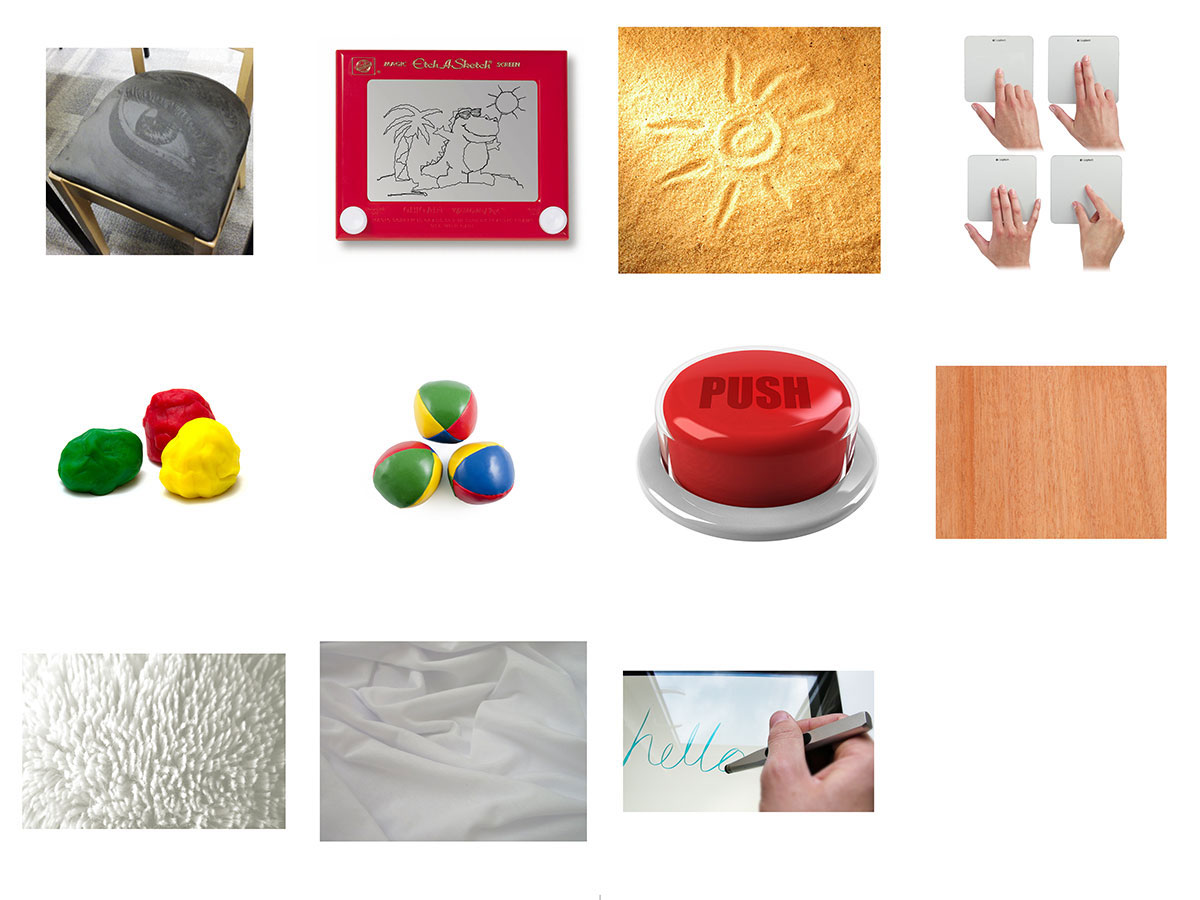
\includegraphics[width=4in]{workshops/technology-cards}
    \caption[A list of inspirational workshop cards.] % in list of figures
  {Cards that were used as inspiration in workshop II.} % beneath the figure
  \label{ch:workshops:technology-cards}
\end{figure}



\subsection{Discussion}


\section{Discussion}

\todo{Conventions and the familiarity of the home ... Dindler, 2010 - Lerdahl, Bell, Ehn...} Were we successful in defamiliarising the home setting???

